\chapter{Introduction}



\section{Motivation} \label{sec:Einl:Motivation}
The finite element method (FEM) is a numerical technique for finding approximate solutions to boundary value problems for partial differential equations. FEM contains linear FEM and non-linear FEM. 
Linear analysis follows the equation $K\cdot D = F$, which K stands for stiffness matrix, D stands for  displacement and F stands for force. It means that the correlation of force and displacement is linear. This relation between force and displacement is only valid for material that has elastic linear property. But in real situation, elastic material such as steel has also non- linear region. (see the Figure \ref{fig: nonlinear}). The property is elastic linear,  until at yield point, the steel is yielding and become non-linear. Non-linear cases include geometry non- linear and material non- linear. The example in Figure \ref{fig: nonlinear} just describes a non-linear case and it is also the main topic in this thesis. This thesis will only focus on nonlinear FEM. In engineering and science in general, FEM helps tremendously in producing strength visualization and it is also possible to lead engineer for minimizing weight, materials and costs. The accuracy of solution are only limited by the quality of model and by the available computational power.  Since the computational power has been improved enormously, FEM software offers a wide range of simulation of complex model designs and analysis of a system.  \newline
AMfe is a nonlinear finite element code for structural application at chair of applied mechanics in Technical University of Munich. AMfe Toolbox is developed in Python and Fortran. Python is a high-level, interpreted and dynamically-typed programming language.  There are many numerical packages built on Python, such as Numpy, Scipy, Pandas. These packages provide high-performance, easy to use data structures, which just match for a FEM developing work. And because Python is a high-level programming language, it makes less time to develop the code, but on the other hand, it is slow for repeated execution of low-level task. Each Python operation comes with a small type-checking overhead, and with many repeated small operation, this overhead becomes significant. For that reason, the part of code are rewritten in Fortran. Fortran is a general-purpose, imperative programming language that is especially suited to numeric computation and scientific computing. So this combination obtain the advantage from both of them- easy to develop in Python and fast numeric computation in Fortran. The aim of AMfe Toolbox is to solve and analyse FEM problems, especially structural mechanical problems.
It contains several modules with different functions to solve problems step by step. A simple structure of AMfe are depicted in Figure \ref{fig: Overview2}. Displacement, stress and strain are three important factors for structural mechanical engineering. The function for calculation of nodal displacements is completed in AMfe Toolbox. Stress and strain calculation are still empty. Stress and strain calculations are of interest because in structural mechanical analysis and design for geometry the stresses are often very important to the engineer. For that reason, functions for solving of stress and strain will be added in AMfe Toolbox. When stress is able to export, a research to increase the accuracy of results is worthy of consideration. To improve the accuracy of the results, stress recovery is a approach to extrapolate the element solution to nodal solution. The goal is to get as much accuracy from the computed displacements while keeping the computational effort reasonable. When the most important functions are done and works well, it is time to check if AMfe Toolbox export the reasonable results. The results of stress and strain from AMfe Toolbox will be compared with a commercial FEM software - ANSYS. The compare of each element type will be recorded. 

\begin{figure}
	\begin{center}
		\includegraphics[width=12cm,clip]{nonlinear.pdf}			
		\caption{Stress-strain curve for steel} \label{fig: nonlinear}
	\end{center}
\end{figure}

\section{Structure of Study}

\begin{figure}
	\begin{center}
		\includegraphics[width=12cm,clip]{Overview.pdf}			
		\caption{Flow chart of structure} \label{fig: Overview}
	\end{center}
\end{figure}

\begin{figure}
	\begin{center}
		\includegraphics[width=12cm,clip]{Overview2.pdf}			
		\caption{Overview of AMfe structure} \label{fig: Overview2}
	\end{center}
\end{figure}

This study can be divided into three parts.  Figure \ref{fig: Overview} shows the flow chart of structure in this study. The first part is marked with green box. The main job for this part is to export data of meshed geometry by using ANSYS Parametric Design Language(APDL) code and import them into AMfe Toolbox. This procedure called Pre-Processing which is the first step in solving a problem in Finite Element Analysis. This step also ensures the both analysis with same set of elements and nodes. After that it is the processing step, which is marked with yellow box. AMfe Toolbox has several modules with different functions. These modules combine with each other and provides all the calculation function for processing. This study is focusing on calculating stress and strain. The last part marked with blue colour is to check the accuracy of stress and strain with using different types of elements.

\chapter{Numerical Aspect for Finite Element Formulation}
\section{Shape Function}
\subsection{Quadrilateral Elements}
To get the approximate solution (position, displacement, stress and strain) in structural mechanical field is the goal of AMfe Code.  The approximation is basically depended on shape function $N$. The standard approach for the definition of shape functions is to chose them as simple polynomials which are associated to nodes. One element includes $n$ nodes and $n$ shape functions, where the $i$-th shape function takes the value 1 at the $i$-th node in reference coordinates, then the $j$-th shape function can be written like this: \\

\begin{center}
	if $j$ = $i$ then $N_j\left(\hat{\xi_i}\right) = 1$ \\
	if $j$ $\neq$ $i$ then $N_j\left(\hat{\xi_i}\right) = 0$
\end{center}

for $i$,$j$ = 1,...,n. \\
In Figure \ref{fig: shape_func}, linear, quadratic shape function are shown together with corresponding node positions. When it comes to a element with three nodes, as shown in the right of Figure \ref{fig: shape_func}. For each shape functions, there are three restrictions:

\begin{figure}
	\begin{center}
		\includegraphics[width=10cm,clip]{shape_func.pdf} 		
		\caption{Linear shape function and quadratic shape function.} \label{fig: shape_func}	
	\end{center}
\end{figure}

\begin{center}
	$N_1\left(\hat{\xi_1} = -1\right) = 1$, $N_1\left(\hat{\xi_2} = 0\right) = 0$, $N_1\left(\hat{\xi_3} = 1\right) = 0$;\\
	$N_2\left(\hat{\xi_1} = -1\right) = 0$, $N_2\left(\hat{\xi_2} = 0\right) = 1$, $N_2\left(\hat{\xi_3} = 1\right) = 0$;\\
	$N_3\left(\hat{\xi_1} = -1\right) = 0$, $N_3\left(\hat{\xi_2} = 0\right) = 0$, $N_3\left(\hat{\xi_3} = 1\right) = 1$
\end{center}

In general quadratic polynomial, the shape functions have three coefficients, and it can be constructed as follows:
\begin{center}
	$p_{quad}\left(\xi\right) = c_0 + c_1\xi + c_2\xi^2$
\end{center}

Lagrange polynomials are a general class of polynomials with the node association property: a Lagrange polynomial $l_k^n-1$ (in one coordinate $\xi$) of order $n-1$ passes through $n$ nodes with coordinates $\bar{\xi^j}\left(j = 1,...,n\right)$ of which the single node $k$ evaluates unity $\left(l_k^{n-1} \left(\bar{\xi^k}\right)=1\right)$ and every other node results in zero $\left(l_k^{n-1} \left(\bar{\xi^k}\right)=0  \quad \text{for all} \quad j \neq k\right)$ .

\begin{center}
	$l_k^{n-1} \left( \xi \right) = \prod_{j = 1, j \neq k}^{n} \frac{\xi - \bar{\xi^1}}{\bar{\xi^k - \bar{\xi^j}}} = \frac{\left(\xi - \bar{\xi}^1\right)\cdot\cdot\cdot \left( \xi - \bar{\xi}^{k-1}\right) \left(\xi - \bar{\xi}^{k+1}\right)\cdot\cdot\cdot \left(\xi -\bar{\xi}^n\right)}{\left(\bar{\xi}^k - \bar{\xi}^1\right)\cdot\cdot\cdot \left( \bar{\xi}^k - \bar{\xi}^{k-1}\right) \left(\bar{\xi}^k - \bar{\xi}^{k+1}\right)\cdot\cdot\cdot \left(\bar{\xi}^k -\bar{\xi}^n\right)}$ \\[4mm] \quad $k = 1,2....,n$
\end{center}
For instance linear, i.e. order 1, Lagrange polynomials are achieved with $n-1=1$ $\Rightarrow$ $n=2$ nodes. Using $\bar{\xi}^1 = -1$ and $\bar{\xi}^2 = +1$ results in: $l_1^1\left(\xi\right) = -1/2\left(\xi - 1\right)$ and $l_2^1\left(\xi\right) = 1/2\left(\xi + 1\right)$.
Then the linear shape functions can be simply constructed as $N_1 =l_1^1 = 1/2\left(1-\xi\right)$ and $N_2 = l_2^1 = 1/2\left(1+\xi\right)$.

\subsection{Triangular and Tetrahedral Elements}
Due to the higher flexibility of triangles and tetrahedra for meshing complex geometries, they are often preferred over quadrilaterals or hexahedral. The shape functions are given in an analogous method, but they are expressed in area and volume coordinates, respectively. Figure \ref{tri&tet} shows the geometries and shape functions. These coordinates represent area and volume fractions, a visualization is given below:
\begin{center}
	$L_1 = \frac{\text{area}P23}{\text{area}123}$, \quad $V_1 = \frac{\text{area}P234}{\text{area}1234}$ \\[4mm]
	$\sum L_i = 1$ \quad\quad $\sum V_i = 1$
\end{center}

\begin{figure}
	\begin{center}
		\includegraphics[width=11cm,clip]{Tri&Tet.pdf}			
		\caption{triangular and tetradral elemnets.} \label{fig: tri&tet}
	\end{center}
\end{figure}

\section{Non- linear Element Formulation}
\subsection{Discretization of the Displacement Field}
After meshing of the geometry, displacement field $u$ can be discretized by inserting shape function $N$. Firstly, we introduce the nodal displacement $d^e$ to save displacements at each node of the considered element for each spatial direction.
In elastic materials, through the elastic constitutive equations can be derived that stresses $\sigma$ are directly related to strains $\varepsilon$ at each point:
\begin{equation}
\sigma = E\varepsilon
\end{equation}
It follows that the stress calculation procedure begins with strain calculation, and that the accuracy of stresses depends on that of strains. In the following sections, we focus our attention on two-dimensional isoparametric elements, as the calculation of strains, stresses and axial forces in bar elements is strightforward. Suppose that we have solved the master stiffness equations. 
\begin{equation}
Ku = f
\end{equation}
for the node displacements $u$. To calculate strains and stresses we perform a loop over all defined elements. Let $\varepsilon$ be the element index of a specific two-dimensional isoparametric element encoun- tered during this loop, and $u(\varepsilon)$ the vector of computed element node displacements. The strains at any point in the element can be related to these displacements as 
\begin{equation}
\varepsilon = Bu(\varepsilon) 
\end{equation}
where $B$ is the strain-displacement matrix assembled with the x and y derivatives of the element shape functions evaluated at the point where we are calculating strains. The corresponding stresses are given by 
\begin{equation}
\sigma = E\varepsilon = EBu 
\end{equation}
In the applications it is of interest to evaluate and report these stresses at the element nodal points located on the corners and possibly midpoints of the element. These are called element nodal point stresses.
It is important to realize that the stresses computed at the same nodal point from adjacent elements will not generally be the same, since stresses are not required to be continuous in displacement- assumed finite elements. This suggests some form of stress averaging can be used to improve the stress accuracy, and indeed this is part of the stress recovery technique further. The results from this averaging procedure are called nodal point stresses.

\section{Non-linear Formulation of Strain and Stress}
This section provides an introduction to the most common model and simulation technique for both 2D and 3D solid bodies in Non-Finite-Element-Method. According to Rutzmoser \cite{Johannes} ,in the first part of this introduction, we will pick a fictional 3D element with five nodes as object of study. The coordinate system is based on three coordinate:$\xi_1$, $\xi_2$ and $\xi_3$. Therefore the shape function of this element can be ordered in Voigt notation as follows:
\begin{equation}
 \textbf{\textit{N}}\left(\xi\right) = \begin{pmatrix}
 N_1\left(\xi\right)           \\[0.3em]
 N_2\left(\xi\right)            \\[0.3em]
 N_3\left(\xi\right)           \\[0.3em]
 N_4\left(\xi\right)         \\[0.3em]
 N_5\left(\xi\right)                            
\end{pmatrix}
\end{equation}
We can denote the coordinate of element as vector $\textbf{\textit{X}}^e$. The columns of $\textbf{\textit{X}}^e$ stands for axis direction and the rows of $\textbf{\textit{X}}^e$ stands for index of nodes. The matrix of $\textbf{\textit{X}}^e$ is shown as:
\begin{equation}
\textbf{\textit{X}}^e = \begin{pmatrix}
X_1 & Y_1 & Z_1           \\[0.3em]
X_2 & Y_2 & Z_2             \\[0.3em]
X_3 & Y_3 & Z_3           \\[0.3em]
X_4 & Y_4 & Z_5          \\[0.3em]
X_5 & Y_5 & Z_6                            
\end{pmatrix}
\end{equation}	
The coordinates $\textbf{\textit{X}}$ of element in the initial configuration relies on the local coordinate of element $\xi$ and the shape function $\textbf{\textit{N}}$. It can be described as:
\begin{equation}
\textbf{\textit{X}}  \left(\xi\right) = \begin{pmatrix}
X \\
Y \\
Z
\end{pmatrix} = \left(\textbf{\textit{X}}^e\right)^T N = \begin{pmatrix}
X_1 & X_2 & X_3 & X_4 & X_5 \\
Y_1 & Y_2 & Y_3 & Y_4 & Y_5 \\
Z_1 & Z_2 & Z_3 & Z_4 & Z_5
\end{pmatrix} \begin{pmatrix}
N_1 \\
N_2 \\
N_3 \\
N_4 \\
N_5 
\end{pmatrix}
\end{equation} 
The displacements $\textbf{\textit{u}}$ of any points of the element are interpolated from the nodal coordinate, just like it was done previous for the coordinates $\textbf{\textit{X}}$. So the displacements field can be shown as:
\begin{equation}
\textbf{\textit{u}}\left(\xi\right) = \begin{pmatrix}
u_x\left(\xi\right) \\
u_y\left(\xi\right) \\
u_z\left(\xi\right) 
\end{pmatrix} = \left(\textbf{\textit{u}}^e\right)^T N = \begin{pmatrix}
u_{x1} & u_{x2} & u_{x3} & u_{x4} & u_{x5} \\
u_{y1} & u_{y2} & u_{y3} & u_{y4} & u_{y5} \\
u_{z1} & u_{z2} & u_{z3} & u_{z4} & u_{z5}
\end{pmatrix} \begin{pmatrix}
N_1 \\
N_2 \\
N_3 \\
N_4 \\
N_5 
\end{pmatrix}
\end{equation}
This approach is called isoparametric concept, that is possible to present all the parameters in Element. The method to calculate the magnitude of parameter in element is using the known value of parameters at every nodes and the shape function. An example of displacements can be formed like this:
\begin{equation}
\frac{\partial \textbf{\textit{u}}}{\partial \textbf{\textit{X}}} = \left(\textbf{\textit{u}}^e\right)^T \frac{\partial \textbf{\textit{N}}}{\partial \textbf{\textit{X}}} = \left(\textbf{\textit{u}}^e\right)^T \tilde{\textbf{\textit{B}}_0}
\end{equation}
The deviation of parameter can be passed to the shape function. By using this approach, we can define a new term $\tilde{\textbf{\textit{B}}_0} = \frac{\partial \textbf{\textit{u}}}{\partial \textbf{\textit{X}}}$. The expand of $\tilde{\textbf{\textit{B}}_0}$ can be derived as:
\begin{equation} \label{eq: B_0}
\frac{\partial \textbf{\textit{N}}}{\partial \textbf{\textit{X}}} = \tilde{\textbf{\textit{B}}_0} = \begin{pmatrix}
\frac{\partial N_1}{\partial X} & \frac{\partial N_1}{\partial Y} & \frac{\partial N_1}{\partial Z} \\
\frac{\partial N_2}{\partial X} & \frac{\partial N_2}{\partial Y} & \frac{\partial N_2}{\partial Z} \\
\frac{\partial N_3}{\partial X} & \frac{\partial N_3}{\partial Y} & \frac{\partial N_3}{\partial Z} \\
\frac{\partial N_4}{\partial X} & \frac{\partial N_4}{\partial Y} & \frac{\partial N_4}{\partial Z} \\
\frac{\partial N_5}{\partial X} & \frac{\partial N_5}{\partial Y} & \frac{\partial N_5}{\partial Z} \\
\end{pmatrix} = \frac{\partial \textbf{\textit{N}}}{\partial \boldsymbol{\xi}} \frac{\partial \boldsymbol{\xi}}{\partial \textbf{\textit{X}}}
\end{equation}
The first term of equation \ref{eq: B_0} can be directly presented with shape function. It is shown as:
\begin{equation}
\frac{\partial \textbf{\textit{N}}}{\partial \boldsymbol{\xi}} = \begin{pmatrix}
\frac{\partial N_1}{\partial \xi_1} & \frac{\partial N_1}{\partial \xi_2} & \frac{\partial N_1}{\partial \xi_3} \\
\frac{\partial N_2}{\partial \xi_1} & \frac{\partial N_2}{\partial Y
	\xi_2} & \frac{\partial N_2}{\partial \xi_3} \\
\frac{\partial N_3}{\partial \xi_1} & \frac{\partial N_3}{\partial \xi_2} & \frac{\partial N_3}{\partial \xi_3} \\
\frac{\partial N_4}{\partial \xi_1} & \frac{\partial N_4}{\partial \xi_2} & \frac{\partial N_4}{\partial \xi_3} \\
\frac{\partial N_5}{\partial \xi_1} & \frac{\partial N_5}{\partial \xi_2} & \frac{\partial N_5}{\partial \xi_3} \\
\end{pmatrix}
\end{equation}
The second term $\frac{\partial \boldsymbol{\xi}}{\partial \textbf{\textit{X}}}$ is not straightforward to obtain. On the other hand it is much more easier to get the matrix $\frac{\partial \textbf{\textit{X}}}{\partial \boldsymbol{\xi}}$. This matrix is called Jocobian matrix $\textbf{\textit{J}}$, which is a matrix of $\boldsymbol{\xi}$ with respect to $x$. The inverse Jocobian are denoted as $\textbf{\textit{J}}^{-1}$, which is the second term. \\
The deformation gradient $\textbf{\textit{F}} = \textbf{\textit{H}} + \textbf{\textit{I}}$ can be defined through the help matrix $\textbf{\textit{H}} = \frac{\partial \textbf{\textit{u}}}{\partial \textbf{\textit{X}}} = \left(\textbf{\textit{u}}^e\right)^T \tilde{\textbf{\textit{B}}_0}$, which describes the mapping of an infinitesimal fiber in the initial state to its new position in the current configuration. Then, the Green-Lagrange strain tensor can be also formed as:
\begin{equation}
\textbf{\textit{E}} = \frac{1}{2} \left(\textbf{\textit{H}} + \textbf{\textit{H}}^T + \textbf{\textit{H}}^T \textbf{\textit{H}}\right)
\end{equation}
\begin{equation} \label{eq: E_eq}
\textbf{\textit{E}} = \frac{1}{2} \left(\textbf{\textit{F}}^T \textbf{\textit{F}} - \textbf{\textit{I}}\right)
\end{equation}
The help matrix $\textbf{\textit{H}}$ can be expressed more detailed as:
\begin{equation} \label{eq: Help_matrix}
\textbf{\textit{H}} = \frac{\partial \textbf{\textit{u}}}{\partial \textbf{\textit{X}}} = \frac{\partial \textbf{\textit{u}}}{\partial \boldsymbol{\xi}} \frac{\partial \boldsymbol{\xi}}{\partial \textbf{\textit{X}}} = \left(\textbf{\textit{u}}^e\right)^T \frac{\partial \textbf{\textit{N}}}{\partial \boldsymbol{\xi}} \left[ \left(\textbf{\textit{X}}^e\right)^T \frac{\partial \textbf{\textit{N}}}{\partial \boldsymbol{\xi}}\right]^{-1}
\end{equation}
It is possible to calculate stress $\textbf{\textit{S}}$ while strain is presented. One simply constitutive equation between stress $\textbf{\textit{S}}$ (2. Piola-Kirchhoff-Stress tensor) and $\textbf{\textit{E}}$ (Green-Lagrange-Strain tensor) can be formulated as:
\begin{equation}
\textbf{\textit{S}} = \textbf{\textit{C}} : \textbf{\textit{E}}
\end{equation}
The result of stress is subsequently transfer into the degree of freedom at each nodes. The principle for calculation of stress can be formulated as follows:\\
In the total Lagrange approach, the principle of virtual work represents that the internal stress work $\delta \textbf{\textit{W}}_{int} = \int \boldsymbol{\sigma} : \delta \boldsymbol{\epsilon} \mathrm{d}\Omega_0 = \int \textbf{\textit{S}} : \delta \textbf{\textit{E}} \mathrm{d}\Omega_0$ equals the external node force $\delta \textbf{\textit{W}}_{ext} = \left(\delta \textbf{\textit{u}}^{e,v}\right)^T \textbf{\textit{f}}_{nl}^v$
\begin{equation} \label{eq: W}
\delta \textbf{\textit{W}} = \delta \textbf{\textit{W}}_{ext} = \left(\delta \textbf{\textit{u}}^{e,v}\right)^T \textbf{\textit{f}}_{int}^v = \int \textbf{\textit{S}} : \delta \textbf{\textit{E}} \mathrm{d}\Omega_0 = \int \left( \delta \textbf{\textit{E}}^v\right)^T \textbf{\textit{S}}^v \mathrm{\Omega_0}
\end{equation}
The internal deformation work can be computed by matrix-vector-product in voigt-notation or direct product of two matrix with notation (:). Now, we evaluate the variation of Green-Lagrange strain tensor $\delta \textbf{\textit{E}}$. From equation \ref{eq: E_eq}, it is obvious that the variation of tensor $\delta \textbf{\textit{E}}$ is determined by the variation of deformation gradient. According to above equation \ref{eq: Help_matrix}, the variation of deformation gradient can be transformed as:
\begin{equation}
\delta \textbf{\textit{F}} = \delta \textbf{\textit{H}} = \left(\delta \textbf{\textit{u}}^e\right)^T \frac{\delta \textbf{\textit{N}}}{\delta \textbf{\textit{X}}} = \left(\delta \textbf{\textit{u}}^e\right)^T \tilde{\textbf{\textit{B}}_0}
\end{equation}
Consequently, the variation of tensor $\delta \textbf{\textit{E}}$ as:
\begin{equation}
\delta \textbf{\textit{E}} = \frac{1}{2} \left(\delta \textbf{\textit{F}}^T \textbf{\textit{F}} + \textbf{\textit{F}}^T \delta F \right)
\end{equation}
Green-Lagrange-Strain are often represented in voigt-notation because of the complex matrix form in computer programming. Then, $\delta \textbf{\textit{E}}^v$ can be coupled with $\textbf{\textit{B}}_0$-matrix as:
\begin{equation} \label{eq: E_voigt}
\delta \textbf{\textit{E}}^v = \textbf{\textit{B}}_0 \delta \textbf{\textit{u}}^{e,v}
\end{equation} 
The entries of $\textbf{\textit{B}}_0$ will be packed as a black box and direct implemented in the FEM simulation. Gathering the equation \ref{eq: W} and equation \ref{eq: E_voigt}, the non-linear force results in:
\begin{equation}
\delta \textbf{\textit{W}} = \left(\delta \textbf{\textit{u}}^{e,v}\right)^T \textbf{\textit{f}}_{int}^v = \int \left(\delta \textbf{\textit{E}}^v\right)^T \textbf{\textit{S}}^v \mathrm{d}\Omega_0 = \left( \delta \textbf{\textit{u}}^{e,v}\right)^T \int \textbf{\textit{B}}_0^T \textbf{\textit{S}}^v \mathrm{d}\Omega_0
\end{equation}
\begin{equation}
\textbf{\textit{f}}_{int}^v = \int \textbf{\textit{B}}_0^T \textbf{\textit{S}}^v \mathrm{d}\Omega_0
\end{equation}
The non-linear internal force of element concerning to coordinate of node can be integrated by $\textbf{\textit{B}}_0$-martrix with second Piola-Kirchhoff-Stress tensor in voigt-notation. To obtain the tangential stiffness matrix, it is necessary to calculate the partial derivative of internal force $\textbf{\textit{f}}_{int}^v$ respect to the nodal degree of freedom $\textbf{\textit{u}}^{e,v}$:
\begin{equation} \label{K}
\frac{\partial \textbf{\textit{f}}_{int}^v}{\partial \textbf{\textit{u}}^{e,v}} = \textbf{\textit{K}} = \int \frac{\partial \textbf{\textit{B}}_0^T}{\partial \textbf{\textit{u}}^{e,v}} \textbf{\textit{S}}^v \mathrm{d}\Omega_0 + \int \textbf{\textit{B}}_0^T \frac{\partial \textbf{\textit{S}}^v}{\partial \textbf{\textit{u}}^{e,v}} \mathrm{d}\Omega_0 = \textbf{\textit{K}}_{geo} + \textbf{\textit{K}}_{mat}
\end{equation}
Stiffness can be divide into two term, one for material stiffness matrix $\textbf{\textit{K}}_geo$, which is shown as:
\begin{equation}
\textbf{\textit{K}}_{mat} = \int \textbf{\textit{B}}_0^T \frac{\partial \textbf{\textit{S}}^v}{\partial \textbf{\textit{u}}^{e,v}}\mathrm{d}\Omega_0 = \int \textbf{\textit{B}}_0^T\frac{\partial \textbf{\textit{S}}^v}{\partial \textbf{\textit{E}}^v} \frac{\partial \textbf{\textit{E}}^v}{\partial \textbf{\textit{u}}^{e,v}} \mathrm{d}\Omega_0 = \int \textbf{\textit{B}}_0^T \textbf{\textit{C}}^{SE} \textbf{\textit{B}}_0 \mathrm{d}\Omega_0
\end{equation}
The derivative of stress respect to strain is considered as Tangent-Modulus $\textbf{\textit{C}}^{SE} = \frac{\partial \textbf{\textit{S}}^v}{\partial \textbf{\textit{E}}^v}$ by constitutive equation. The derivative of strain is $\textbf{\textit{B}}_0$ as determined in equation \ref{eq: E_eq}. \\
The geometrical stiffness matrix is much more complex to derive. In a word, the internal work from equation \ref{eq: W} is reformulated by concerning relation between the deformation gradient and continuum mechanics $\textbf{\textit{P}} = \textbf{\textit{S}}\textbf{\textit{F}}^T$:
\begin{equation}
\delta \textbf{\textit{W}} = \textbf{\textit{u}}^e : \textbf{\textit{f}}_{int} = \int \delta \textbf{\textit{F}}^T : \textbf{\textit{P}} \mathrm{d}\Omega_0 = \int \delta \textbf{\textit{F}}_{ij} \textbf{\textit{P}}_{ji} \mathrm{d}\Omega_0
\end{equation}
The variation of deformation gradient $\delta \textbf{\textit{F}} = \delta \textbf{\textit{u}}^{eT} \textbf{\textit{B}}_0$. In index-notation form it can be written as $\delta \textbf{\textit{F}}_{ij} = \delta \textbf{\textit{u}}_{ki}^e \tilde{\textbf{\textit{B}}_{kj}^0}$. Then, the internal force in matrix notation can be derived as:
\begin{equation}
\delta \textbf{\textit{W}} = \delta u^e : \textbf{\textit{f}}_{int} = \textbf{\textit{u}}_{ki}^e \textbf{\textit{f}}_{ki}^{int} = \int \delta \textbf{\textit{F}}_{ji} \textbf{\textit{P}}_{ij} \mathrm{d}\Omega_0 = \delta \textbf{\textit{u}}_{ki}^e \int \tilde{\textbf{\textit{B}}_{kj}^0} \textbf{\textit{P}}_{ji}\mathrm{d}\Omega_0 = \delta \textbf{\textit{u}}^e : \int \tilde{\textbf{\textit{B}}_0} \textbf{\textit{P}} \mathrm{d}\Omega_0
\end{equation}
\begin{equation}
\textbf{\textit{f}}_{int} = \int \tilde{\textbf{\textit{B}}_0} \textbf{\textit{P}} \mathrm{d}\Omega_0
\end{equation}
The tangential stiffness matrix is defined by changing the force vector, which is determined over time concerning with the velocity of nodal displacement $\dot{\textbf{\textit{u}}^e}$. Because Jacobi-Matrix is relative complex to build. Therefore, the derivative of internal force $\dot{\textbf{\textit{f}}_{int}}$in time as follows:
\begin{equation} \label{eq: f_int}
\dot{\textbf{\textit{f}}_{int}} = \int \tilde{\textbf{\textit{B}}_0} \dot{\textbf{\textit{S}}} \textbf{\textit{F}}^T \mathrm{d}\Omega_0 + \int \tilde{\textbf{\textit{B}}_0} \textbf{\textit{S}} \dot{\textbf{\textit{F}}^T} \mathrm{d}\Omega_0
\end{equation}
The fist term conresponds to material stiffness, becasue the time derivative of second Piola-Kirchhoff-Stress tensor is related with time-dependent part. And the second term conresponds to geometrical stiffness as shown in equation \ref{K}. Becase the time derivative $\dot {\textbf{\textit{F}}}$ equals $\dot{\textbf{\textit{u}}^e}^T \tilde{\textbf{\textit{B}}_0}$, equation\ref{eq: f_int} can be transformed as:
\begin{equation}
\dot{\textbf{\textit{f}}}_{int,geo} = \int \tilde{\textbf{\textit{B}}}_0 \textbf{\textit{S}} \tilde{\textbf{\textit{B}}}_0 \mathrm{\Omega_0} \dot{\textbf{\textit{u}}}^e
\end{equation}
The geometrical stiffness matrix is given, because the temporal variation of non-linear force is coupled with the displacements over the tangential stiffness matrix.
\begin{equation}
\dot{\textbf{\textit{f}}}_{int,geo} = \textbf{\textit{K}}_{geo} \dot{\textbf{\textit{u}}}^e =\int \tilde{\textbf{\textit{B}}}_0 \textbf{\textit{S}} \tilde{\textbf{\textit{B}}}_0 \mathrm{\Omega_0} \dot{\textbf{\textit{u}}}^e
\end{equation}
The last step to determine the non-linear force and the tangential stiffness matrix is to integrate on domain $d\Omega_0$. There are two concept for this integration to mention: the first one is transformation from domain $d\Omega_0$ to reference coordinate system:
\begin{equation}
\int {\textbf{\textit{f}}}\left(x\right) \mathrm{d}\Omega = \int {\textbf{\textit{f}}}\left(x\right) \frac{\partial \boldsymbol{\xi}}{\partial \boldsymbol{\xi}} \mathrm{d}\Omega = \int {\textbf{\textit{f}}}\left(x\right) \frac{\partial \Omega}{\partial \boldsymbol{\xi}} \mathrm{d}\boldsymbol{\xi} = \int {\textbf{\textit{f}}}\left(x\right) det \left(\frac{\partial X}{\partial \boldsymbol{\xi}}\right) \mathrm{d}\boldsymbol{\xi}
\end{equation}
For the transformation of integration, it is necessary to adapt the bound of integration. It is in FEM a pleasant benefit, its advantage is the new bound of integration is the standard bound of reference element. So it is easier to determine the bound of integration. And the Jocobi-matrix is ready to use, because we have once the inverse of Jocobi-matrix calculated.

\subsection{Gauss Integration}
Numerical integration plays a important role in finite element. Gauss integration, as an efficient approach compared to other numerical integration, integrate a function $\textbf{\textit{f}}(\boldsymbol{\xi})$ on the spatial domain $\Omega$ is replaced by a summation of certain function values at the so-called Gauss points $\tilde{\boldsymbol{\xi}}$ which are each multiplied by a scalar (weight) $\boldsymbol{\omega}$.  In total $numgp_1$ $\times$ $numggp_2$ $\times$ $numgp_3$ Gauss points are used:
\begin{equation}
\int \limits_E {\textbf{\textit{f}}} \left(\boldsymbol{\xi}\right) \mathrm{d\boldsymbol{\xi_1}}\mathrm{d\boldsymbol{\xi_2}}\mathrm{d\boldsymbol{\xi_3}} = \displaystyle\sum_{i=1}^{numgp_1}\displaystyle\sum_{j=1}^{numgp_2} \displaystyle\sum_{k=1}^{numgp_3} f\left(\tilde{\boldsymbol{\xi_1^i}}\tilde{\boldsymbol{\xi_2^j}}\tilde{\boldsymbol{\xi_3^k}}\right)\cdot w_1^i w_2^j w_3^k
\end{equation}
In which we used corresponding weights for each of the three spatial directions. This allows to use Gauss points coordinates and weights tabulated for the one-dimensional case. The location and weights of these points can be given analytically in Table \ref{tab: Gauss table}.
	
\begin{table}
	\begin{center}
		\caption{Gauss-Legendre points and weights}\label{tab: Gauss table}
		\begin{tabular}{cccc}
			$numgp$         & i & $\tilde{\xi^i}$ & $\omega^i$  \\ \hline
			1                           &1& 0 & 2   \\ \hline
			\multirow{2}{*}{2} &1& $-1/\sqrt{3}$ & 1   \\
			&2& $+1/\sqrt{3}$ & 1   \\ \hline
			\multirow{3}{*}{3} &1& $-\sqrt{3/5}$ &5/9 \\
			&2& 0                &8/9 \\
			&3& $+\sqrt{3/5}$ &5/9 \\ \hline
			\multirow{4}{*}{4}&1& $-\sqrt{\left(15+\sqrt{120}\right)/35}$ & $\left(18-\sqrt{30}\right)/36$ \\
			&2& $-\sqrt{\left(15-\sqrt{120}\right)/35}$ & $\left(18+\sqrt{30}\right)/36$ \\
			&3& $+\sqrt{\left(15-\sqrt{120}\right)/35}$ & $\left(18+\sqrt{30}\right)/36$ \\
			&4& $+\sqrt{\left(15+\sqrt{120}\right)/35}$ & $\left(18-\sqrt{30}\right)/36$ \\ \hline
			\multirow{5}{*}{5}&1& $-1/3\sqrt{5+2\sqrt{10/7}}$ & $\left(332-13\sqrt{70}\right)/900$ \\
			&2& $-1/3\sqrt{5-2\sqrt{10/7}}$ & $\left(332+13\sqrt{70}\right)/900$ \\
			&3& 0 & 128/255 \\
			&4& $+1/3\sqrt{5-2\sqrt{10/7}}$ & $\left(332+13\sqrt{70}\right)/900$ \\
			&5& $+1/3\sqrt{5+2\sqrt{10/7}}$ & $\left(332-13\sqrt{70}\right)/900$ \\ \hline
		\end{tabular}
	\end{center}	
\end{table}

\section{Extrapolation from Gauss Points}
\subsection{Quad4}
This will be explained for the four-node bilinear quadrilateral. The normal Gauss integration rule for element stiffness evaluation is 2 $\times$ 2, as illustrated in Figure \ref{fig: Quad4_1}. The stresses are calculated at the Gauss points, which are identified as $k_1^G$, $k_2^G$, $k_3^G$ and $k_4^G$ in Figure \ref{fig: Quad4_1}. Point $k_i^G$ is closest to node $k_i^E$ so it is seen that Gauss point numbering essentially follows element node numbering in the counterclockwise sense. The natural coordinates of these points are listed in Table \ref{tab: Quad4}. The stresses are evaluated at these Gauss points by passing these natural coordinates to the shape function subroutine. Then each stress component is “carried” to the corner nodes $k_1^E$ through $k_4^E$ through a bilinear extrapolation based on the computed values at $k_1^G$ through $k_4^E$. To understand the extrapolation procedure more clearly it is convenient to consider the region bounded by the Gauss points as an “internal element” or “Gauss element”. This interpretation is depicted in Figure \ref{fig: Quad4_1}. The Gauss element, denoted by (G), is also a four-node quadrilateral. The coordinate of node for element and Gauss element can be represented as $k_i^G$ and $k_i^E$, respectively. Its quadrilateral (natural) coordinates are denoted by $\xi^{\prime}$ and $\eta^{\prime}$.  These are linked to $\xi^{\prime}$ and $\eta^{\prime}$ by the simple relations from Gauss-Legendre quadrature in Table \ref{tab: Quad4}.
\begin{equation}
k_i^G = \frac{k_i^E}{\sqrt{3}},\quad
k_i^E= k_i^G\sqrt{3}
\end{equation}

\begin{figure}[h]
	\begin{center}
		\includegraphics[width=8cm,clip]{Quad4_1.pdf}			
		\caption{Quad4 in element coordinate and Gauss element coordinate.}	\label{fig: Quad4_1}
	\end{center} 
\end{figure}

\begin{figure}[h]
	\begin{center}
		\includegraphics[width=8cm,clip]{Quad4_2.pdf}			
		\caption{Equation of side opposite corner 1 for Quad4.} \label{fig: Quad4_2}
	\end{center} 
\end{figure}

\begin{table}
	\centering
	\caption{Natural Coordinate of Quad4}
	\label{tab: Quad4}
	\begin{tabular}{p{1cm}ccccp{1cm}cccc}			
		\hline
		Corner node\centering& $\xi$& $\eta$& $\xi'$& $\eta'$& Gauss node\centering& $\xi$& $\eta$& $\xi'$& $\eta'$ \\
		\hline
		1\centering& -1& -1& $-\sqrt{3}$& $-\sqrt{3}$& 1'\centering& 1/$\sqrt{3}$& -1/$\sqrt{3}$& -1& -1 \\
		2\centering& +1& -1& $+\sqrt{3}$& $-\sqrt{3}$& 2'\centering& 1/$\sqrt{3}$& 1/$\sqrt{3}$& +1& -1 \\
		3\centering& +1& +1& $+\sqrt{3}$& $+\sqrt{3}$& 3'\centering& 1/$\sqrt{3}$& 1/$\sqrt{3}$& +1& +1\\
		4\centering& -1& +1& $-\sqrt{3}$& $+\sqrt{3}$& 4'\centering& -1/$\sqrt{3}$& 1/$\sqrt{3}$& -1& +1\\
		\hline
	\end{tabular}
\end{table}		

The element geometry and natural coordinates are shown in Figure \ref{fig: Quad4_1}. Only one type of node (corner)  and associated shape function is present. Consider node 1 as typical. Inspection of Figure \ref{fig: Quad4_2} suggests trying

\begin{equation} \label{eq: Quad4_1}
N_1^e = c_1L_{2-3}L_{3-4}
\end{equation}
This plainly vanishes over nodes 2, 3 and 4, and can be normalized to unity at node 1 by adjusting $c_1$. By construction it vanishes over the sides 2-3 and 3-4 that do not belong to 1. The equation of side 2-3 is $\xi = 1$, or $\xi - 1 = 0$. The equation of side 3-4 is $\eta = 1$, or $\eta - 1 = 0$. Replacing in Equation (\ref{eq: Quad4_1}) yields

\begin{equation}
N_1^e\left(\xi, \eta\right) = c_1 \left( \xi -1 \right) \left( \eta - 1\right) = c_1 \left(1 - \xi\right) \left( 1 - \eta \right)
\end{equation}
To find $c_1$, evaluate at node 1, the natural coordinates of which are $\xi = \eta = -1$:

\begin{equation}
N_1^e \left(-1, -1 \right) = c_1 \times 2 \times 2 = 4c_1 = 1
\end{equation}

Hence $c_1 = \frac{1}{4}$ and the shape functions is

\begin{equation}
N_1^e = \frac{1}{4} \left(1 - \xi\right) \left( 1 - \eta\right)
\end{equation}

For the other three nodes the procedure is the same, traversing the element cyclically. It can be verified that the general expression of the shape functions for this element is 

\begin{equation}
N_i^e = \frac{1}{4} \left( 1 + \xi_i \xi\right) \left(1 + \left(\eta_i \eta\right)\right)
\end{equation}

Following this general expression, the shape functions of Node 2, 3 and 4 are demonstrated as

\begin{equation}
N_2^e = \frac{1}{4} \left(1 + \xi\right) \left( 1 - \eta\right)
\end{equation}

\begin{equation}
N_3^e = \frac{1}{4} \left(1 + \xi\right) \left( 1 + \eta\right)
\end{equation}

\begin{equation}
N_4^e = \frac{1}{4} \left(1 - \xi\right) \left( 1 + \eta\right)
\end{equation}

When we have all the shape function for Gauss element, it is able to extrapolate the component(stress, strain, etc) from Gauss points $k_i^G$ to corner nodes $k_i^E$. According to \ref{tab: Quad4} and \ref{fig: Quad4_1}, we have the corner nodes in Gauss coordinate: $k_1^E(-\sqrt{3}, -\sqrt{3})$ , $k_2^E(\sqrt{3}, -\sqrt{3})$, $k_3^E(\sqrt{3}, \sqrt{3})$, $k_4^E(\sqrt{3}, \sqrt{3})$. The extrapolation process is to replace all the corner nodes in Gauss coordinate into the shape function of each Gauss points. Then we obtain:
\begin{equation}
\begin{pmatrix}
w_1 \\
w_2 \\
w_3 \\
w_4 \\
\end{pmatrix} = \begin{pmatrix}
1 + \frac{1}{2} \sqrt{3} & -\frac{1}{2} &  1 - \frac{1}{2} \sqrt{3} &  -\frac{1}{2}       \\[0.3em]
-\frac{1}{2} & 1 + \frac{1}{2} \sqrt{3} & -\frac{1}{2} &  1 - \frac{1}{2} \sqrt{3}            \\[0.3em]
1 - \frac{1}{2} \sqrt{3} & -\frac{1}{2}  & 1 + \frac{1}{2} \sqrt{3} &  -\frac{1}{2}         \\[0.3em]
-\frac{1}{2} &  1 - \frac{1}{2} \sqrt{3} & -\frac{1}{2} &   1 + \frac{1}{2} \sqrt{3}                             
\end{pmatrix} \begin{pmatrix}
{w_1}' \\
{w_2}' \\
{w_3}' \\
{w_4}' \\
\end{pmatrix}
\end{equation}	
Here $w'$ means strains and stresses for our case. So the $w'$ part can be written as:
\begin{equation}
\begin{pmatrix}
{w_1}' \\
{w_2}' \\
{w_3}' \\
{w_4}' \\
\end{pmatrix} = \begin{pmatrix}
\epsilon_{1xx} & \epsilon_{1yy} & \epsilon_{1zz} & 2\epsilon_{1yz} & 2\epsilon_{1xz} & 2\epsilon_{1xy}   \\
\epsilon_{2xx} & \epsilon_{2yy} & \epsilon_{2zz} & 2\epsilon_{2yz} & 2\epsilon_{2xz} & 2\epsilon_{2xy}   \\
\epsilon_{3xx} & \epsilon_{3yy} & \epsilon_{3zz} & 2\epsilon_{3yz} & 2\epsilon_{3xz} & 2\epsilon_{3xy}   \\
\epsilon_{4xx} & \epsilon_{4yy} & \epsilon_{4zz} & 2\epsilon_{4yz} & 2\epsilon_{4xz} & 2\epsilon_{4xy}   \\
\end{pmatrix}
\end{equation}

\begin{equation}
\begin{pmatrix}
{w_1}' \\
{w_2}' \\
{w_3}' \\
{w_4}' \\
\end{pmatrix} = \begin{pmatrix}
\sigma_{1xx} & \sigma_{1yy} & \sigma_{1zz} & \sigma_{1yz} & \sigma_{1xz} & \sigma_{1xy}   \\
\sigma_{2xx} & \sigma_{2yy} & \sigma_{2zz} & \sigma_{2yz} & \sigma_{2xz} & \sigma_{2xy} \\
\sigma_{3xx} & \sigma_{3yy} & \sigma_{3zz} & \sigma_{3yz} & \sigma_{3xz} & \sigma_{3xy} \\
\sigma_{4xx} & \sigma_{4yy} & \sigma_{4zz} & \sigma_{4yz} & \sigma_{4xz} & \sigma_{4xy}  \\
\end{pmatrix}
\end{equation}

\subsection{Quadrangle with quadratic shape function and eight nodes: Quad8}
For Quad8(Quadrangle with quadratic shape function and eight nodes) we have various choice for the type of Gauss element.  We usually use four, eight and nine nodes for three quadrilateral elements. Here we introduce the Gauss element with nine nodes. The nine-nodes quadrilateral has three types of shape functions, which are associated with corner, midside nodes and center node, respectively. The element coordinate and Gauss element coordinate are illustrated in Figure \ref{fig: Quad8_1} \\
The lines whose product is used to construct three types of shape functions are illustrated in Figure  for nodes 1, 5 and 9, respectively. The technique has been sufficiently illustrated in previous examples. Here the summary of calculation for nodes 1, 5 and 9, which are taken as representatives of the three types: The three types of shape function are represented in Figure \ref{fig: Quad8_2}.

\begin{equation} \label{eq: Quad8_1}
N_1^e = c_1 L_{2-3}L_{3-4}L_{5-7} L_{6-8} = c_1 \left(\xi - 1\right) \left(\eta -1\right) \xi \eta
\end{equation}

\begin{equation} \label{eq: Quad8_2}
N_5^e = c_5L_{2-3} L_{1-4} L_{6-8} L_{3-4} = c_5 \left(\xi -1 \right) \left( \xi +1\right) \eta \left( \eta -1\right) = c_5 \left(1-\xi^2\right) \eta \left(1 - \eta\right)
\end{equation}

\begin{equation} \label{eq: Quad8_3}
N_9^e = c_9L_{1-2} L_{2-3} L_{3-4} L_{4-1} = c_9 \left(\xi -1 \right) \left( \eta - 1\right) \left(\xi + 1\right) \left( \eta + 1\right) = c_9 \left(1-\xi^2\right) \left(1 - \eta^2\right)
\end{equation}

Imposing the normalization conditions result in:

\begin{center}
	$c_1 = \frac{1}{4}$, \quad $c_5 = -\frac{1}{2}$, $c_9 = 1$
\end{center}

By following this approach all the shape functions can be calculated

\begin{equation}
N_1 = \frac{1}{4} \left(\xi - 1\right) \left( \eta -1 \right) \cdot\xi \cdot\eta
\end{equation}

\begin{equation}
N_2 = \frac{1}{4} \left(\xi + 1\right) \left( \eta -1 \right) \cdot\xi \cdot\eta
\end{equation}

\begin{equation}
N_3 = \frac{1}{4} \left(\xi + 1\right) \left( \eta + 1 \right) \cdot\xi \cdot\eta
\end{equation}

\begin{equation}
N_4 = \frac{1}{4} \left(\xi - 1\right) \left( \eta + 1 \right) \cdot\xi \cdot\eta
\end{equation}

\begin{equation}
N_5 = \frac{1}{2} \left(1 + \xi \right) \left( 1 + \xi \right)  \left( \eta - 1\right) \cdot\eta
\end{equation}

\begin{equation}
N_6 = \frac{1}{2} \left(1 + \eta \right) \left( 1 - \eta \right)  \left( \xi + 1\right) \cdot\xi
\end{equation}

\begin{equation}
N_7 = \frac{1}{2} \left(1 + \xi \right) \left( 1 + \xi \right)  \left( \eta + 1\right) \cdot\eta
\end{equation}

\begin{equation}
N_8 = \frac{1}{2} \left(1 + \eta \right) \left( 1 - \eta \right)  \left( \xi - 1\right) \cdot\xi
\end{equation}

\begin{equation}
N_9 = \left(1 + \xi \right) \left( 1 - \xi \right)  \left( 1 + \eta \right) \left(1 - \eta \right)
\end{equation}

Same as Quad4, the extrapolation function can be expressed by replacing corner nodes in Gauss coordinate into the shape function of Gauss points:
\begin{equation}
\begin{pmatrix}
w_1 \\
w_2 \\
w_3 \\
w_4 \\
w_5 \\
w_6 \\
w_7 \\
w_8 \\
\end{pmatrix} = \begin{pmatrix}
a_1 & a_2 &  a_3 &  a_2 & a_4 & a_5 & a_5 & a_4 & a_6       \\[0.3em]
a_2 & a_1 &  a_2 &  a_3 & a_4 & a_4 & a_5 & a_5 & a_6       \\[0.3em]
a_3 & a_2 &  a_1 &  a_2 & a_5 & a_4 & a_4 & a_5 & a_6       \\[0.3em]
a_2 & a_3 &  a_2 &  a_1 & a_5 & a_5 & a_4 & a_4 & a_6       \\[0.3em]
0     & 0    &  0     &  0     & a_7 & 0     & a_8 & 0    & a_9       \\[0.3em]
0     & 0    &  0     &  0     & 0    & a_7 & 0      & a_8 & a_9       \\[0.3em]
0     & 0    &  0     &  0     & a_8 & 0    & a_7 & 0      & a_9       \\[0.3em]
0     & 0    &  0     &  0     & 0     & a_8 & 0 & a_7     & a_9       \\[0.3em]                    
\end{pmatrix} \begin{pmatrix}
{w_1}' \\
{w_2}' \\
{w_3}' \\
{w_4}' \\
{w_5}' \\
{w_6}' \\
{w_7}' \\
{w_8}' \\
{w_9}'
\end{pmatrix}
\end{equation}	
\begin{align*}
a_1 = +2.1869398 \\
a_2 = +0.2777778 \\
a_3 = +0.0352824 \\
a_4 = -0.9858870 \\
a_5 = -0.1252241 \\
a_6 = +0.4444444 \\
a_7 = +1.4788331 \\
a_8 = +0.1878361 \\
a_9 = -0.6666666
\end{align*}



\begin{figure}[h]
	\begin{center}
		\includegraphics[width=10cm,clip]{Quad8_1.pdf}			
		\caption{Quad8 in element coordinate and Gauss element coordinate.} \label{fig: Quad8_1}
	\end{center} 
\end{figure}

\begin{figure}[h]
	\begin{center}
		\includegraphics[width=6cm,clip]{Quad8_2.pdf} 
		\includegraphics[width=6cm,clip]{Quad8_3.pdf}	
		\includegraphics[width=6cm,clip]{Quad8_4.pdf}
		\caption{Equation of side opposite corner 1 for Quad8.} \label{fig: Quad8_2}	
	\end{center} 
\end{figure}

\subsection{Triangle with three nodes: Tri3}
The geometry of the 3-node triangle shown in Figure \ref{fig: Tri3_1} is specified by the location of its three corner nodes on the $\left\{x, y\right\}$ plane. The shape function for triangular element has a different form, which compares with quadrilateral elements. The three shape functions have the simply own coordinates - the triangular coordinates: $N_i = \xi_i$ for $i = 1, 2, 3.$ The shape function can be derived from a method as follows: The equation of triangle side opposite to node $i$ is $L_{j-k} = \xi_i = 0$, where $j$ and $k$ are the cyclic permutations of $i$. Here symbol $L_{j-k}$ denotes the left hand side of the homogeneous equation of the natural coordinate line that passes through node points $j$ and $k$. See Figure \ref{fig: Tri3_2} for $i = 1$, $j=2$ and $k = 3$. Hence the obvious suppose is:
\begin{equation}
N_i^e = c_iL_i
\end{equation}
To find $c_1$, evaluate $N_1^e\left(\xi_1, \xi_2, \xi_3\right)$ at node 1. The triangular coordinates of this node are $\xi_1$ =1, $\xi_2 = \xi_3 = 0$.  $N_1^e\left(1,0,0\right) = c_1 \times 1 = 1$. so $c_1 = 1$ and analogically $c_2 = 1$, $c_3 = 1$

\begin{equation}
N_1^e = L_1 , \quad N_2^e = L_2, \quad N_3^e = L_3
\end{equation}

Quantities that are closely linked with the element geometry are best expressed in triangular co- ordinates. On the other hand, quantities such as displacements, strains and stresses are usually expressed in the Cartesian system. Thus we need transformation equations through which it is possible to pass from one coordinate system to the other.
Cartesian and triangular coordinates are linked by the relation.

\begin{equation}
\begin{bmatrix}
1 \\
x \\
y \\
\end{bmatrix}
= 
\begin{bmatrix}
1&1&1 \\
x_1&x_2&x_2 \\
y_1&y_2&y_2 \\
\end{bmatrix}
\begin{bmatrix}
\xi_1 \\
\xi_2 \\
\xi_3 \\
\end{bmatrix}
\end{equation}

\begin{equation}
\begin{bmatrix}
\xi_1 \\
\xi_2 \\
\xi_3 \\
\end{bmatrix}
= 
\frac{1}{2A}\begin{bmatrix}
x_2y_3-x_3y_2&y_2-y_3&x_3-x_2 \\
x_3y_1-x_1y_3&y_3-y_1&x_1-x_3 \\
x_1y_2-x_2y_1&y_1-y_2&x_2-x_1 \\
\end{bmatrix}
\begin{bmatrix}
1\\
x \\
y \\
\end{bmatrix}
= 
\frac{1}{2A}\begin{bmatrix}
2A_{23}&y_{23}&x_{32} \\
2A_{31}&y_{31}&x_{13} \\
2A_{12}&y_{12}&x_{21} \\
\end{bmatrix}
\begin{bmatrix}
1 \\
x \\
y \\

\end{bmatrix}
\end{equation}


By using the same approach as quadrilateral elements, the extrapolation of Tri3 can be expressed as:


\begin{figure}[h]
	\begin{center}
		\includegraphics[width=8cm,clip]{Tri3_1.pdf}			
		\caption{Tri3 in element coordinate and Gauss element coordinate.} \label{fig: Tri3_1}
	\end{center} 
\end{figure}

\begin{table}
	\centering
	\caption{Natural Coordinate of Tri3} \label{tab: Tri3}
	\begin{tabular}{p{1cm}ccccp{1cm}cccc}	
		
		\hline
		Corner node\centering& $\xi$& $\eta$& $\xi'$& $\eta'$& Gauss node\centering& $\xi$& $\eta$& $\xi'$& $\eta'$ \\
		\hline
		1\centering& -1& -1& -5/3& -5/3& 1'\centering& -2/3& -2/3& -1& -1 \\
		2\centering& +1& -1& +7/3& -5/3& 2'\centering&+1/3 & -2/3& +1& -1 \\
		3\centering& -1& +1& -5/3& +7/3& 3'\centering& -2/3& +1/3& -1& +1\\
		\hline
		
	\end{tabular}
\end{table}			



\begin{figure}[h]
	\begin{center}
		\includegraphics[width=6cm,clip]{Tri3_2.pdf}			
		\caption{Equation of side opposite corner 1 for Tri3.} \label{fig: Tri3_2}
	\end{center} 
\end{figure}

\subsection{Second order triangle with six nodes: Tri6}
The geometry of the six-node quadratic is shown in Figure XXX. Inspection reveals two types of nodes: corners(1, 2 and 3) and midside nodes(4, 5 and 6). For both cases it is necessary to product the two linear functions in the triangular coordinates because the shape function should be quadratic. These functions are illustrated in Figures XXX for corner node 1 and midside node 4, respectively. \\
For corner node 1, inspection of Figure \ref{fig: Tri6_2} at top left side suggests trying
\begin{equation}
N_1^e = c_1L_{2-3}L_{4-6}
\end{equation}
$N_1^e$ will vanish over 2-5-3 and 4-6. This makes the function zero at node 2,3,4,5,6, as is obvious upon inspection of Figure XXX, while being nonzero at 1. The value can be adjusted to be unity if $c_1$ is appropriately chosen. The equations of the lines that appear (XXX equation upper) are
\begin{equation}
L_{2-3}: \xi_1 = 0, \quad L_{4-6}: \xi_1 - \frac{1}{2} = 0
\end{equation}
Replacing into (eq upper upper)

\begin{equation}
N_1^e = c_1\xi_1 \left(\xi_1 - \frac{1}{2}\right)
\end{equation}
Same as triangle with three nodes, $N_1^e\left(1,0,0\right) = c_1 \times 1 \times \frac{1}{2} = 1$. Then $c_1 = 2$ can be calculated and finally 

\begin{equation}
N_1^e = 2\xi_1\left(\xi_1 - \frac{1}{2}\right) = \xi_1 \left(2 \xi_1 -1 \right)
\end{equation} 

For midside node 4, inspection of Figure XXX suggests trying

\begin{equation}
N_4^e = c_4L_{2-3}L_{1-3}
\end{equation}
The equation of sides $L_{2-3}$ and $L_{1-3}$ are $\xi_1 = 0$ and $\xi_2 = 0$, respectively. Therefore $N_4^e\left(\xi_1, \xi_2, \xi_3\right) = c_4\xi_1\xi_2$. To find $c_4$, evaluate this function at node 4, the triangular coordinates of which are $\xi_1 = \xi_2 = \frac{1}{2}$,$\xi_3 = 0$. Then $N_4^e\left(\frac{1}{2}, \frac{1}{2}, 0\right) = c_4 \times \frac{1}{2} \times \frac{1}{2} = 1$. Hence $c_4 = 4$, which the shape function gives

\begin{equation}
N_4^e = 4\xi_1\xi_2
\end{equation}
The rest shape function can be calculated by using same approach. 
\begin{center}
	
\end{center}

\begin{figure}[h]
	\begin{center}
		\includegraphics[width=8cm,clip]{Tri6_1.pdf} 		
		\caption{Tri6 in element coordinate and Gauss element coordinate.} \label{fig: Tri6_1}	
	\end{center} 
\end{figure}

\begin{figure}[h]
	\begin{center}
		\includegraphics[width=6cm,clip]{Tri6_2.pdf}		
		\includegraphics[width=6cm,clip]{Tri6_3.pdf}		
		\caption{Equation of side opposite corner 1 for Tri6.} \label{fig: Tri6_2}
		
	\end{center} 
\end{figure}


\subsection{Tetraeder element with four nodes: Tet4}

\begin{figure}[h]
	\begin{center}
		\includegraphics[width=8cm,clip]{Tet4_1.pdf}			
		\caption{Tri4 in element coordinate and Gauss element coordinate.}
	\end{center} 
\end{figure}

\begin{table}
	\centering
	\caption{Tetrahedral Coordinate of Tet4}
	\begin{tabular}{ccccccccc}			
		\hline
		Corner node\centering& L1& L2& L3& L4& L1'& L2'& L3'& L4'\\ \hline
		1\centering& 1& 0& 0& 0& $\alpha$& $\beta$& $\beta$& $\beta$\\
		2\centering& 0& 1& 0& 0& $\beta$& $\alpha$& $\beta$& $\beta$\\
		3\centering& 0& 0& 1& 0& $\beta$& $\beta$& $\alpha$& $\beta$\\
		4\centering& 0& 0& 0& 1& $\beta$& $\beta$& $\beta$& $\alpha$\\
		\hline
		Gauss node\centering& L1& L2& L3& L4& L1'& L2'& L3'& L4' \\ \hline
		1'\centering& $\alpha$& $\beta$& $\beta$& $\beta$& 1& 0& 0& 0  \\
		2'\centering&$\beta$ & $\alpha$& $\beta$& $\beta$& 0& 1& 0& 0 \\
		3'\centering& $\beta$& $\beta$& $\alpha$& $\beta$& 0& 0& 0& 1\\
		4'\centering& $\beta$& $\beta$& $\beta$& $\alpha$& 0& 0& 0& 1\\
		\hline
		$\alpha$ = 0.58541020; $\beta$ = 0.13819660&&&&&&&&\\
		\hline 		    
	\end{tabular}	
\end{table}		

\chapter{Programming Implementation}
\section{Pre-Processing}
The purpose of Pre-Processing is to build a numerical model and export as two lists- node list and element list.  The data of model are ultimately imported into AMfe Toolbox. ANSYS Parametric Design Language (APDL) code is the tool to create a meshed geometry in ANSYS. A simple meshed geometry are shown in Figure \ref{fig: muster}. Task step for building model contains a series of related path. An example of a path step is: 

\begin{center}
	\large{\textbf{Geometry $\Rightarrow$ Element Type $\Rightarrow$ Material $\Rightarrow$ Mesh
			$\Rightarrow$ Boundary Condition  }}
\end{center}

After building the model, numerical data can be exported as node list and element list. Node list contains coordinate all the nodes of geometry. Element list are formed with the attributes of each elements and the index of node with belongs to element. The element attributes are assigned to different parts of model by 'pointing' to the appropriate entries in the element list. The pointers are simply a set of reference numbers that include  the element index (ELEM), material number (MAT), element type number (TYP), real constant set number (REAL), a coordinate system number (ESY) and section ID number (SEC). Connecting with the example in Figure \ref{fig: muster}, both lists are depicted in Table \ref{tab: node_list} and Table \ref{tab: element_list}. The numerical information of both lists are captured with regular expression approach and stored in AMfe Toolbox. For different data it is necessary to store in specific data type. Coordinate of each node and the index of nodes from elements are stored as Numpy array. NumPy is the fundamental package for scientific computing with Python. The advantage of Numpy for storage of node and element information depends on its efficient multi-dimensional container of generic data. It contains a powerful N-dimensional array object and sophisticated (broadcasting) functions. Moreover, it is possible for integrating Fortran code. General attributes of element can be stored as a efficient form- Pandas DataFrames. Pandas is a powerful data analysis toolkit, which provides fast, flexible, and expressive data structures designed to make working with relational or labeled data both easy and intuitive. Pandas DataFrames is a two-dimensional size-mutable, potentially heterogeneous tabular data structure with labeled axes (rows and columns). Arithmetic operations align on both row and column labels. This format can be thought of as a dictionary-like container for Series objects. 

\begin{figure}
	\begin{center}
		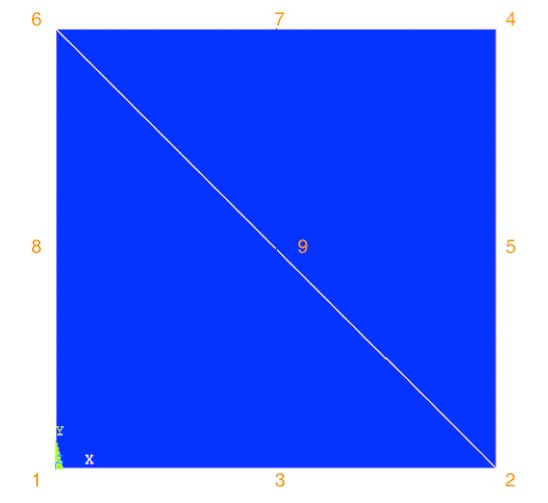
\includegraphics[width=10cm,clip]{muster.png} 			
		\caption{A simple meshed geometry} \label{fig: muster}
	\end{center}
\end{figure}

\begin{table}
	\begin{center}
		\caption{Node list exported from ANSYS}\label{tab: node_list}
		\begin{tabular}{ ccccccc }
			\hline			
			NODE & X & Y & Z & THXY & THYZ & THZX\\ \hline
			1 & 0.0000 & 0.0000 & 0.0000 & 0.00 & 0.00 & 0.00 \\
			2 & 50.000 & 0.0000 & 0.0000 & 0.00 & 0.00 & 0.00 \\
			3 & 25.000 & 0.0000 & 0.0000 & 0.00 & 0.00 & 0.00 \\
			4 & 50.000 & 50.000 & 0.0000 & 0.00 & 0.00 & 0.00 \\
			5 & 50.000 & 25.000 & 0.0000 & 0.00 & 0.00 & 0.00 \\
			6 & 0.0000 & 50.000 & 0.0000 & 0.00 & 0.00 & 0.00 \\
			7 & 25.000 & 50.000 & 0.0000 & 0.00 & 0.00 & 0.00 \\
			8 & 0.0000 & 25.000 & 0.0000 & 0.00 & 0.00 & 0.00 \\
			9 & 25.000 & 25.000 & 0.0000 & 0.00 & 0.00 & 0.00 \\
			\hline  
		\end{tabular}	
	\end{center}
\end{table}

\begin{table}
	\begin{center}
		\caption{Element list exported from ANSYS}\label{tab: element_list}
		\begin{tabular}{ cccccccccccc }
			\hline			
			ELEM & MAT & TYP & REL & ESY & SEC & Node & Node  & Node & Node & Node & Node\\ \hline
			1 & 1 & 1 & 1 & 0 & 1 & 6 & 2 & 4 & 9 & 5 & 7 \\
			2 & 1 & 1 & 1 & 0 & 1 & 6 & 1 & 2 & 8 & 3 & 9 \\
			\hline  
		\end{tabular}		
	\end{center}	
\end{table}
\cite[p. 18]{bibid}
Interelement Averaging can be as future research ..
\cite[p. 1-10]{Johannes}